\chapter{The Analysis Process}

For each MIDlet suite, the \textbf{analysis process} consists of the
sequential execution of phases. Each phase is dedicated to the control
of particular characteristics, and its scope is either global
(the analysis target is the entire MIDlet suite) or local (per MIDlet
analysis). In that sense, in its simplest use the \ma should be seen as a
\textbf{sequencer of phases} over a given MIDlet suite. This is
illustrated in figure \ref{figSAA}, where analysis parameters are at least a JAR
file and a profile.


\begin{figure}[h] 
\begin{center}
\scalebox{0.6}{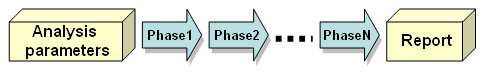
\includegraphics{figures/Sequencer1D}}
\end{center}
\caption{A single analysis process execution}
\label{figSAA}
\end{figure}

\begin{figure}[t]
\begin{center}
\scalebox{0.58}{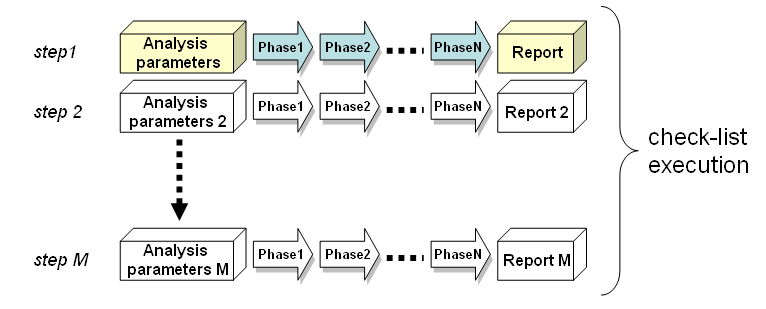
\includegraphics{figures/Sequencer2D}}
\end{center}
\caption{A check-list execution}
\label{figSeq2D}
\end{figure}


So far, only three phases are available but we plan to add new ones in
a future release of the tool. Besides, note that executing a
check-list means to run the analysis process several times
in sequence, as shown on figure \ref{figSeq2D}.


\section{The Descriptors Conformity Phase (MIDP)}
The Descriptors Conformity phase checks the wellformed-ness and completeness of the
descriptors that can be associated with a MIDlet suite: 

\begin{itemize}
\item the JAD file (optional)
\item the JAR manifest file (mandatory), which contains similar information to the
  JAD's.
\end{itemize}

Some rules apply all the time, while others apply only if
the two files are present since they are related to their mutual
consistency (remember the presence of a JAD is optional). The main
problems that can be reported are listed below.


\subsection{Problems that may happen in any descriptor (JAD or
  Manifest)}
\begin{itemize}
\item Mandatory attribute missing
\item Incorrect value for an attribute
\item Double definition of an attribute
\item MIDlet declaration is malformed. Three parameters (name, icon,
  class name) are expected; however the icon parameter may be empty.
\item Name for a MIDlet missing
\item Class name for a MIDlet missing
\item Class for a MIDlet declared in the descriptor actually does not exist
  in the JAR file
\item Icon for a MIDlet declared in the descriptor actually does not exist
  in the JAR file
\item Icon for a MIDlet declared in the descriptor actually does not seem to
  be a PNG file 
\end{itemize}

\subsection{Problems specific to the JAD}
\begin{itemize}
\item Can't read certificate \emph{n} in path (\emph{m}).
\end{itemize}

\subsection{Problems that may happen if the two descriptors are provided}
\begin{itemize}
\item Mandatory attribute defined in none of the descriptors
\item The JAR file size and the value indicated in the JAD differ
\item Name for a MIDlet differs from the JAR manifest to the JAD
\item Icon for a MIDlet differs from the JAR manifest to the JAD
\item Class for a MIDlet differs from the JAR manifest to the JAD
\end{itemize}

Some of the checks can be customized. It is possible to add constraints on
midlet names, on actions and suffixes handled by CHAPI,  on URLs handled
by PushRegistry.
It is also possible to restrict the number of visible midlet and to impose
constraints on icon sizes.

% \paragraph{Remark} The descriptors conformity phase is a built-in
% phase of the \ma. As a consequence, rules above currently can't be
% customized by the user (in contrast to the Features Usage phase, which
% can be defined in an analysis profile). Another consequence is that
% the Descriptors Conformity phase is run exactly the same way whatever
% the profile used. We are considering improving that in a future
% release of the tool.

\subsection*{Customize some properties of descriptors}
The descriptors conformity phase checks the conformity of descriptors
according to MIDP 2.0 specification and JAR file specification. Nevertheless,
you can add properties in the security profile that have to be 
verified by descriptors. These properties concern:
\begin{itemize}
  \item Line end separators in the JAD file and in the JAR manifest file.
  \item Order of attributes in the descriptors.
  \item Mandatory and forbidden attributes in these files.
\end{itemize}
This customization is detailed in section \ref{CustoConform} of this document.

\section{Android Manifest}
This phase extracts some useful information from the manifest as stored in the
APK file:
\begin{itemize}
  \item The supported screen sizes and density
  \item The permissions used by the midlet (in red, Android system permissions)
  \item The features required if any 
  \item The SDK requirements if documented.
\end{itemize}
\section{The Static Analysis Phase} 
The static analysis phase was initially centered only around feature usage.  As
this phase involves the building of several complex intermediate models that 
are useful for many useful checks,  it has evolved and now contains other 
analysis not directly related to feature usage.

\subsection{The principle of feature Usage}
The \ma's main purpose is to check whether some particular Java features
are used by the MIDlet, and how. This is called the Features Usage
phase. Technically, a Java feature is one particular method of a
particular Java package. The principle is quite simple:

\begin{itemize}
\item A feature is defined by a method of the MIDP profile (or a related
JSR) and a set of arguments. Methods and their arguments  are
identified and declared in an analysis profile.
\item When you run the analysis process, the tool will look for every
  invocation of that method in the MIDlet, and gather information
  about:
\begin{itemize}
\item Where the call is located in the code.
\item The values taken by the arguments during that call, or returned
  by the call. 
\end{itemize}
\item When the process is done, a report will be produced according to
  the report directives that are specified in the analysis profile. 
\end{itemize}

So, the \ma does not only detect the use of a given feature: it can also
computes an upper approximation of the possible values of the parameters passed
to that method at runtime. 

It is important to understand the kind of approximation
handled by the tool. Matos uses three kinds of abstract values: concatenated 
strings, integers and objects.

The tool has been optimized for handling \textbf{character strings}. Basic
approximations are regular constant strings, the ``unknown object'' 
representing any string and coded as \verb!"\*"! and method calls that  have not
been resolved (when the method is not recognised by Matos) which are represented by
\verb!"\[qualified.methodName\]"!. Backslashes in constant strings are escaped
(\verb!\\!). Those objects can be directly concatenated. For example
\verb!"aa\*bb"! represents any string begining with \verb!"aa"! and ending with
\verb!"bb"!. Approximations are sets of such strings.

Arguments of type \textbf{integer} (\texttt{int}) are computable only if
they appear straight as constants in the MIDlet source code.

Class object can also be tracked if they are created as constants and not
extracted from objects. A class object is represented as the name of the class
between brackets.

Finally other kind of objects are represented by the point where they have been
``allocated''. Those points are represented by the type of object they generate
and a unique identifier (a number). They are refered in results by their number 
and written such as \textbf{[5]}.

To help you distinguish different usage of values generated by the system, this version of Matos distinguishes two kinds of allocation points. Real allocation
points defined by a new expression and fake allocation points corresponding to
the point where a CLDC/MIDP method returns a value to the application. Those
allocation are further defined by the program point where the system method was
called.

A program point is defined as a bytecode offset in a method. It is
written \texttt{offset@signature} where \texttt{signature} is the full
specification of the method.

The syntax for method signature is the following:
\begin{alltt}
\textit{signature} ::= <\textit{qualifiedClassName}:\textvisiblespace\textit{subsignature}>
\textit{subsignature} ::= \textit{type}\textvisiblespace\textit{methodName}(\textit{type},\ldots,\textit{type})
\textit{type} ::= \textit{qualifiedClassName} | void | \textit{basicType}
     |  \textit{type}[]
\end{alltt}
Note that spaces are significant. Do not add spurious spaces when you write
method signatures.

It is important to be able to distinguish the two kinds of allocation points.
Two distinct allocation points corresponding to two new expressions represent
\emph{distinct} live objects. On the other hand two distinct allocation points
where at least one is a program point may represent the same live object. It
depends on the semantics of the system method called but a lot of such methods
produce new objects each time they are called.

\subsection{A typical example}
Imagine you decide in your security policy to reject MIDlets that use
the network by opening HTTP connections. 
In MIDP, opening a connection is done through a call to the generic method
\texttt{Connector.open} method with an address parameter that specifies 
which protocol to use:
\begin{verbatim}
c = Connector.open(``http://www.blablabla.org/example.html'');
\end{verbatim}

The call is dynamically protected in that case by the \emph{Net Access} 
security function group and more specifically by the 
\verb!javax.microedition.io.Connector.http! permission.

The \ma  will locate all invocations of the \texttt{Connector.open}
method, and try to
compute all the possible values of the method's argument, which
contains the target URL. If it turns out that at least one possible
value contains the prefix \texttt{http://}, then the tool will inform
you that the MIDlet violates your policy.

In the security profile, these operations are handled by two specification:
\begin{itemize}
  \item a rule that specifies the method to look at
  \item a report that tells how to analyze the result
 \end{itemize}
The rule is the following:
 \begin{verbatim}
 <rule name="HTTP-R">
 <args class="javax.microedition.io.Connector"
       method="javax.microedition.io.Connection open(java.lang.String)"
       report="HTTP">
       <argument position="0"/>
 </args>
 </rule>
\end{verbatim}
It specifies the method by its class and subsignature and the argument to
analyze. The report to use is identified by its name.

Three kinds of results can
come out of the argument analysis, actually. We give examples below:
\begin{itemize}
\item{\textbf{Full computation}}: \texttt{https://www.blablabla.org/index.html}
\item{\textbf{Partial computation}}: \texttt{ht}\emph{*}, or
  \texttt{http://www.blablabla.org/}\emph{*}\texttt{.mp3}
\item{\textbf{Impossible computation}}: \emph{*}
\end{itemize}

where the star here (\emph{*}) represents the non-computable part of the
string. Why is it not always possible to compute the full value?
It depends on the level of complexity of the application. If too
complex operations are applied to the observed data, the \ma may fail
to understand what's going on. Another simple reason is the fact that 
data may get their value externally: if the MIDlet asks the user to 
enter the entire HTTP URL at runtime, then there is no mean to guess what the
user will type.

We will use the following report:
\begin{verbatim}
<report name="HTTP">
  <pseudoString>
  	<filter name="CAPTURED" pattern="http:.*" verdict="FAILED">
  	  HTTP connection
  	</filter>
  	<filter name="OK" pattern="[^\]*:.*" verdict="PASSED">
  	  Another kind of connection
  	</filter>
  	<filter name="NOT ANALYZED" pattern=".*" verdict="FAILED">
  	  Cannot analyze the scheme of this URL
  	</filter>
  </pseudoString>
</report>
\end{verbatim}
It specifies a sequence of filters. Each filter has a name, a verdict status and
a content printed out. It is applied when the pattern filters the approximation
string computed for the argument. Patterns are specified in POSIX syntax. Note
the use of \verb![^\]*! to capture the absence of uncomputed part in the URL
scheme. We could use smarter patterns as it is sufficient to know that the first
letter is not an 'h' but it would be of little practical use.

\subsection{Further technical details}
Generally speaking, the argument analysis is based
on a computation of the possible values that can be stored at 
different program points, taking into account all possible execution
paths of the program. The computation is actually an upper
approximation of the possible values, with the implicit and safe assumption
that when something can't be computed, then it can be \emph{anything}
at runtime. 

The analysis is a \textbf{static analysis} performed on the
application bytecode: as a result, the \ma never needs to run the
MIDlet, it just reasons about its bytecode, after having built an
abstraction of it. The underlying theory is known as abstract interpretation and
was designed by Patrick and Radhia Cousot but the real tool used here is
a pointer analysis (also known as a points-to analysis).


The main purpose of the arguments analysis is to check the values of
arguments passed to certain methods, but you can also check the return
values of methods, as well as the values taken by certain class fields.
Concretely, the target variables (methods arguments, return values, or
attributes) to be checked are specified in the analysis profile. 

\section{The limits of static analysis}
As said earlier, there are cases where the \ma cannot decide whether or not
a MIDlet satisfies a security property because it cannot analyse the arguments
of a method call. To avoid those cases, it is recommended to impose 
coding constraints to developers of MIDlets so that those limits are 
never encountered in practice.

\subsection{The notion of pseudo-constant}
The main principle is that an argument of a method call whose value creates
a security risk should be \emph{almost} constant. The definition of almost 
has been relaxed in such a way to ease the life of application developers.
We will call pseudo-constants values satisfying the necessary conditions.

A simple (simplistic) definition of a pseudo constant is the following.
A pseudo-constant is an object of type string which is either one of the following:
\begin{itemize}
\item a literal or a field declared as \verb!final static! and initialised according to its definition,
\item a static field \verb!v! of a class or an instance field of an object where the class containing it is a class of the MIDlet (and not of the MIDP profile) and where all the values \verb!c! assigned to the field (\verb!v=c!) are 
pseudo-constants.
\item a variable local to a method where all the values assigned to the 
variable are pseudo-constants
\item a parameter of a method. In that case the corresponding argument in all the calls of this method in the source code of the MIDlet must be a 
pseudo-constant,
\item a call to \verb!new String(c)! where \verb!c! is a pseudo constant.
\end{itemize}
Note that the definition of pseudo-constant is recursive: it uses the notion
of pseudo-constants. So the notion of pseudo-constant is in fact 
quite expressive.

\subsection{Extending the definition of pseudo-constants}
The previous definition is very convenient to specify what is authorized to
developers but it also forbids a lot of practical usage. It can  relaxed
a little further for the \ma:
\begin{itemize}
\item if \verb!c1! and \verb!c2! is a pseudo-constant, then so is their
concatenation defined as \verb!c1 + c2! (but you cannot use an explicit global 
string buffer to create it, because the \ma cannot check if there is not
another thread using the same buffer at the same time);
\item if all the values assigned to the element of an array are pseudo-constants, so is the value of any element of the array, but be careful ! all the uses
are merged in a single one for the analysis.
\end{itemize}

If you want to use the relaxed rules, you must be careful that the average
developer will be able to understand what is authorized and what is forbidden.

As a last warning : when programmers use a global variable with
multiple usages \footnote{for example, if a variable is used to store all the newly created strings}, note that all 
the values of this variable are coalesced into a single
usage pattern by the analysis. This means that some use case may be inferred
by the \ma that do not exist in practice. Nevertheless, this set will always
be finite and the evaluator can usually decide if there is a security
 problem or not by looking at the potential values.

\subsection{Tracking arbitrary objects}
The \ma has been designed to track string constants but it may in fact track any
kind of Java object. Abstract objects correspond to roughly allocation points in
the code. An abstract object is presented in the result has an integer between
brackets. Per se it contains no useful information. But abstract objects may
appear in multiple results. In that case, it means that an object used in a
given call \emph{may} be used in another. 

There is usually an object table dumped after the results of the different
rules. This object table contains a line per abstract object that defines its
exact class (as set at the allocation point) and gives pointers to its different
uses.

It is important to understand the difference between abstract objects that
represent sets of potential live object during a real execution and a real
object. When we see a given abstract object at two different program points, it
does not mean that all live objects abstracted by this abstract object have to
be present at both points. On the other hand, if an abstract object is not
present at a given point, it means that all the real object abstracted cannot be
present at this program point. Even with those limitations, abstract objects are
useful to figure out what kind of relations link the real objects. A simple
example is given on figure \ref{objectImage}, an intent is created with a class
object \verb:Main: it is then given to  \verb!startActivity!. Without the
tracking of the abstract object, it would have been difficult to guess
if the intent using this class did corespond to a service or an activity.

\begin{figure}
\begin{minipage}{13cm}
\textbf{Intent-3}\\
\begin{tabular}{|l|l|}
\hline
Caller:	& com.company.appli.TheNotifitication.onClick \\ \hline
Base:	& [1370]b \\ \hline
Argument 2:	& [com.company.appli.Main] \\ \hline
\end{tabular}\\[0.5cm]
\textbf{Context.startActivity}\\
\begin{tabular}{|l|l|}
\hline
Caller:	com.company.appli.TheNotifitication.onClick \\ \hline
Argument 1:	[1370]a \\ \hline
\end{tabular}\\[0.5cm]
\textbf{Object table}\\
\begin{tabular}{|l|l|}
\hline
\multicolumn{2}{|c|}{android.content.Intent} \\ \hline
[1370]	& a ,b \\ \hline
\end{tabular}
\end{minipage}
\caption{An abstract object example}
\label{objectImage}
\end{figure}
%%% Local Variables: 
%%% mode: latex
%%% TeX-master: "Users-manual"
%%% End: 
